\section{Measurement setup}

\subsection{Device post-processing and packaging}\label{sec:fab-packaging}

Once device fabrication is finished, the sample has to be mounted on a chip carrier and contacted, so we can connect it to our measurement electronics.
% 
Our microwave PCBs are made for \SI{10x10}{\milli\meter} chips.
%
However, in order to better hold on to the chips during fabrication and to enhance the fabrication yield, samples are usually fabricated on larger substrates:
% 
The current bias cavities for the graphene devices presented in Chapters~\ref{chap:gJJ} and \ref{chap:gJJ-CPR} were processed on a \SI{2}{inch} wafer, and the cavities based on aluminum in Chapter~\ref{chap:currentdetection} on \SI{15x15}{\milli\meter} chips.

We dice the chips into the correct dimensions in the very last step, using a \textit{Disco dicer DAD 3220} from \textit{Disco Hi-Tec Europe GmbH}.
% 
To protect the chip from dust during sawing, we spincoat photoresist\footnote{HPR504, \SI{4000}{rpm}, bake \SI{60}{\second} at \SI{100}{\celsius}, approximately \SI{1.2}{\micro\meter} thick} on the chip before dicing.
% 
Good resist-substrate adhesion is important because the water jet used to cool the blade can wash off the resist during dicing otherwise, potentially ruining weeks of delicate work in the cleanroom.
% 
Use of HMDS, or letting the resist sit on the chip to be diced for \SI{1}{\minute} prior to spinning, is therefore strongly recommended.

The silicon chips were diced using a standard NBC blade at \SI{3000}{rpm} and a feed speed of \SI{5}{\milli\meter\per\second}, while for dicing sapphire we used a special diamond blade at \SI{2000}{rpm} and \SI{2}{\milli\meter\per\second}.
% 
For the devices presented in this thesis, we placed the diced chips in teflon holders inside beakers filled with PRS3000, heated the solution to \SI{80}{\celsius} and subsequently put the beaker into an ultrasound bath at maximum power.
% 
After \SI{5}{\minute}, the resist has then come off the sample, and we passed the chip through a series of PRS3000 and IPA baths to wash off any remains, and blow-dried using nitrogen.

% 
The chips are finally glued to the rails of our copper boxes using GE low temperature varnish.
% 
Wirebonding is done using a \textit{Westbond 4000 "E"} system from \textit{West•Bond Inc.} with bond wires from an AlSi alloy (\SI{99}{\percent}-\SI{1}{\percent}).
% 
To ensure good thermalization and electrical contact, we usually used three to four bonds for each bond pad, and as many bonds as would fit on the ground planes.
% 
An example of one of our devices that is mounted and wirebonded in a PCB, ready for measurement can be seen in Fig.~\ref{fig:packaging}.
% 
The connectors to go from the PCB to the outside world are straight plug semi-detent SMP connectors\footnote{19S102-40ML5 straight plug PCB, from \textit{Rosenberger Hochfrequenztechnik GmbH \& Co. KG}}.


\begin{figure}
	\centering
	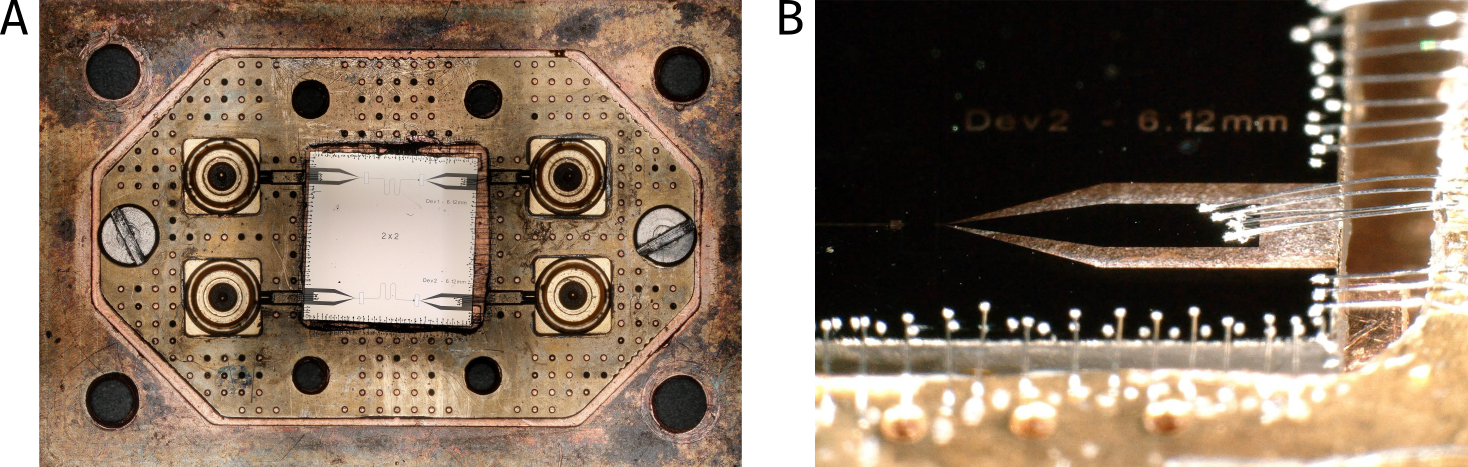
\includegraphics{{chapter-experimental-methods/figs-packaging/packaging.svg}.png}
	\caption{
		\textbf{Device packaging for electrical measurements.}
		% 
		\textbf{(a)} The \SI{10x10}{\milli\meter} chip is mounted and wirebonded to a PCB, that is screwed onto a copper base.
		% 
		The four small holes around the chip are used to screw on a small copper lid, covering the chip.
		% 
		The four big holes at the edge of the copper base are used for mounting the chip in a cryostat, and to hold the top cover in place.
		% 
		Connectors for connecting the PCB to the outside world are surface mount SMP plugs.
		% 
		\textbf{(b)} Close-up of the bottom-right chip area, taken with ring illumination.
		% 
		The substrate is sapphire, hence the chip transparency.
		% 
		In the bottom right corner, one of the copper rails on which the chip sits is visible.
		%
		\textbf{(c)} The individual parts of our sample holder (clockwise):
		%
		PCB for \SI{10x10}{\milli\meter} chips, copper base with rails to mount chip and PCB, small cover, large lid.
		%
		\textbf{(d)} Sample enclosed and mounted in the bottom-loading puck of a \textit{Triton} dilution fridge.
		%
	}
	\label{fig:packaging}
\end{figure}

\subsection{Filtering and attenuation}

\subsubsection{Low frequency interference}

Current and voltage fluctuations originating from room temperature electronics can carry the typical \SI{50}{\hertz} interference (also dubbed \textit{mains hum}), along with other, high-frequency, components.
%
In our lab, we suppress the mains hum by using battery-powered DC electronics for probing and biasing our circuits, the IVVI rack, made at \textit{DEMO}\footnote{Dienst Elektronische en Mechanische Ontwikkeling, \url{https://www.tudelft.nl/demo/}} of TU Delft.
%
The IVVI is controlled via an optical fiber connected to the measurement PCs.

Still, as shown in the Supplementary Material of Chapter~\ref{chap:currentdetection}, to properly suppress the mains hum, battery and mains powered equipment needs to be physically separated from each other.
%
This requires separate grounds between the two, DC blocks for inner and outer conductor attached to all high-frequency lines, as well as placing the IVVI and mains powered equipment on separate racks.

\subsubsection{Thermal excitation}

Thermal excitation can contribute to quasiparticles in the superconductor, meaning introducing a population of unpaired electrons, compared to the lossless Cooper pairs.
%
Table~\ref{tab:fthermal} lists the thermal energies and frequencies corresponding to typical temperatures in our setups.
%
The origin of these excitations in the so-called Johnson-Nyquist noise due to the thermally activated motion of charge carriers in conductors, regardless of applied voltage~\cite{johnsonThermalAgitationElectricity1928,nyquistThermalAgitationElectric1928}.

\begin{table}
	\caption{\textbf{Frequencies and energies of thermal noise.}}
	\label{tab:fthermal}
\begin{tabular}{ccc}
	\hline \hline
	Temperature & Thermal frequency & Thermal energy \\ 
	\hline 
	\SI{300}{\kelvin} & \SI{6.25}{\tera\hertz} & \SI{25.9}{\milli\electronvolt} \\ 
	% \hline 
	\SI{50}{\kelvin} & \SI{1.04}{\tera\hertz} & \SI{4.3}{\milli\electronvolt} \\ 
	% \hline 
	\SI{4}{\kelvin} & \SI{83.3}{\giga\hertz} & \SI{345}{\micro\electronvolt} \\ 
	% \hline 
	\SI{1}{\kelvin} & \SI{20}{\giga\hertz} & \SI{86.2}{\micro\electronvolt} \\ 
	\SI{100}{\milli\kelvin} & \SI{2}{\giga\hertz} & \SI{8.62}{\micro\electronvolt} \\ 
	% \hline 
	\SI{10}{\milli\kelvin} & \SI{208}{\mega\hertz} & \SI{862}{\nano\electronvolt} \\ 
	\hline \hline
\end{tabular}
\end{table}

In order to neglect the influence of thermal effects on our circuits and for the superconductor to be in its thermal ground state, it is necessary to operate the devices at temperatures $T \ll T_c$.
%
Since the superconducting gap voltages of \ce{NbTiN}, \ce{MoRe} and \ce{Al} are \SI{2.3}{\milli\electronvolt}, \SI{1.5}{\milli\electronvolt} and \SI{183}{\micro\electronvolt}, respectively, our experiments require access to the sub-Kelvin regime which is enabled by using dilution refrigerators.
%
However, even with the devices mounted to the base plate of dilution refridgerators (the devices in Chapters~\ref{chap:gJJ} and \ref{chap:gJJ-CPR} in a \textit{Triton 200} from \textit{Oxford Instruments}, the one in Chapter~\ref{chap:currentdetection} in a \textit{LD-400} from \textit{Bluefors}), they still experience some active heat load due to the wiring connecting the sample to the room temperature electronics.
%
This way, thermal noise can couple into the devices.
%
It is therefore vital to suppress this noise by means of signal attenuation before reaching the sample, while not sacrificing too much signal-to-noise ratio.



While attenuating the input lines as much as possible seems to be a good idea at first, this is not necessary because the physical temperature of the lowest fridge stage, in our experiments the base temperature of $T_{\rm MXC}\approx\SI{15}{\milli\kelvin}$, places a lower bound on the sample temperature, and therefore on the required lowest noise temperature.
%
Additionally, due to low electron-phonon coupling at low temperatures, the electrons in the device most likely have a slightly larger temperature than the fridge itself, as cooling becomes inefficient at these temperatures~\cite{giazottoOpportunitiesMesoscopicsThermometry2006}.
%
Cooling below the fridge temperature is possible, but requires nuclear refrigeration in combination with further attenuation and low electron-phonon coupling~\cite{sarsby500MicrokelvinNanoelectronics2020}.
%

Since we will be probing our devices both at DC and with \si{\giga\hertz} frequencies, both low and high frequency lines need to be attenuated separately.
%
Our DC lines are attenuated using home-made two-stage RC and copper powder filters (see Appendix \ref{app:copperpowder} for details).
%
The RC filters have a cutoff frequency $f_{\SI{3}{\decibel}}\approx\SI{30}{\kilo\hertz}$ and suppress higher frequencies up to \SI{20}{\mega\hertz}.
%
Above this range, radiation starts to leak through again, due to stray capacitance of the filter resistors and parasitic inductance of the capacitors, cf. Fig.~\ref{fig:filterDC}(a,b).
%
As shown in Fig.~\ref{fig:filterDC}(b), a two-stage filter has a higher slope, \SI{-40}{dB/decade} compared to \SI{-20}{dB/decade}, while exhibiting only a slightly lower cut-off frequency.
%
The radiation leaking through calls for additional, very high-frequency lowpass filters.
%
We use home-made copper powder filters for this purpose, cf. Fig.~\ref{fig:filterDC}(c,d).
%
These consist of a long PCB trace encased in a copper box, which is filled with copper powder and epoxy, essentially forming a very long and lossy transmission line with very low resistance, suppressing frequencies above a few \SI{100}{\mega\hertz}, as shown in Fig.~\ref{fig:filterDC}(a).

\begin{figure}
	\centering
	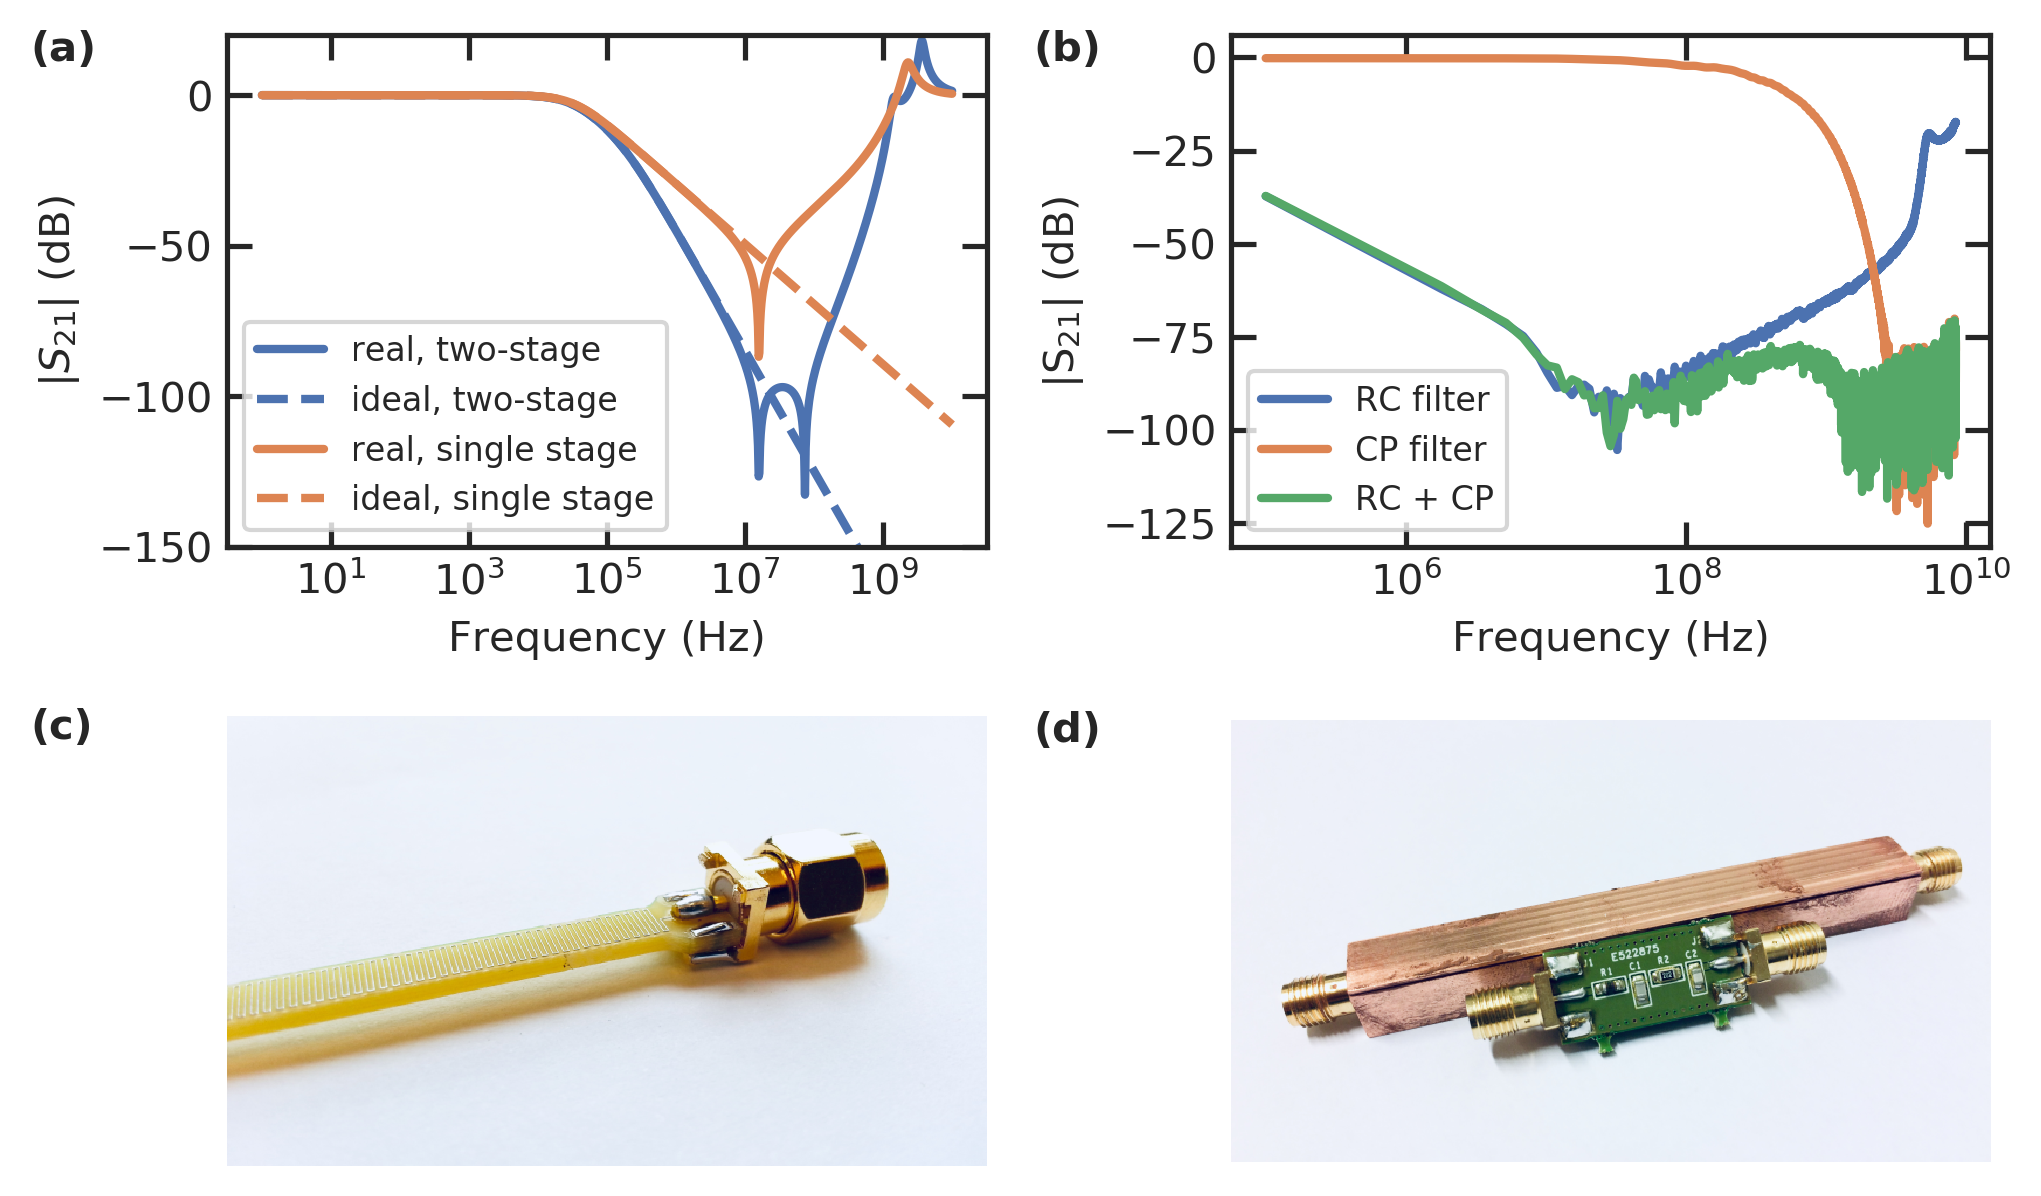
\includegraphics[width=\textwidth]{{chapter-experimental-methods/figs-setup/filterplots/DC_filters}.png}
	\caption{
		\textbf{Electronic noise reduction using low-pass filters.}
		%
		\textbf{(a)} Measured transfer function of combinations of two-stage RC lowpass and copper powder filters.
		%
		Parasitic inductance and capacitances in the RC filter allow radiation to leak through at higher frequencies, which can be suppressed using copper powder filters.
		%
		\textbf{(b)} Simulated transfer function of single (orange) and two-stage (blue) RC low-pass filters.
		%
		Dashed: ideal filter characteristic, solid: realistic behavior with stray capacitance and inductance.
		%
		\textbf{(c)} Copper powder filter PCB with connector, without enclosure.
		%
		The PCB trace is approximately \SI{50}{\centi\meter} long.
		%
		\textbf{(d)} Photograph of a two-stage RC filter of SMD 0812 elements and a fully assembled copper powder filter.
	}
	\label{fig:filterDC}
\end{figure}

We can estimate the effect of attenuation on the electron noise temperature~\cite{krinnerEngineeringCryogenicSetups2019}.
%
With the Bose-Einstein distribution
\begin{align}
n_{\rm BE}(f,T)=\frac{1}{e^{hf/k_B T}-1}\label{eq:nBE}
\end{align}
we can calculate the photon flux at frequency $f$ due to thermal noise coming from $T_1$ transmitted through a bath at $T_2$ with transmission $\tau$ with the rate equation
\begin{align}
n_{\rm ph}(f,T_1,T_2,\tau)=\tau n_{\rm BE}(f,T_1)+(1-\tau)n_{\rm BE}(f,T_2)\label{eq:nphot}
\end{align}
The noise temperature of the corresponding photon flux is then
\begin{align}
T_{n}=\frac{hf}{k_B\ln\left(\frac{n_{\rm ph}+1}{n_{\rm ph}}\right)}
\label{eq:Tnoise}
\end{align}

\begin{figure}
	\centering
	\includegraphics[width=\textwidth]{{chapter-experimental-methods/figs-setup/filterplots/noise_full}.png}
	\caption{
		\textbf{Reducing noise temperature through attenuation.}
		\textbf{(a,b)} Calculated noise temperature \textbf{(a)} and corresponding photon flux \textbf{(b)} of the DC lines using typical low-pass filters for attenuation.
		%
		\textbf{(c,d)} Calculated noise temperature \textbf{(c)} and corresponding photon flux \textbf{(d)} of the RF lines using attenuators of \SI{3}{dB}, \SI{6}{dB}, \SI{10}{dB}, \SI{20}{dB}, and between \SIrange{3}{20}{dB} at the \SI{50}{\kelvin}, \SI{4}{\kelvin}, \SI{1}{\kelvin}, \SI{100}{\milli\kelvin} and \SI{15}{\milli\kelvin} stage, respectively.
	}
	\label{fig:noisefull}
\end{figure}

Our dilution fridges have stages at \SI{50}{\kelvin}, \SI{4}{\kelvin}, \SI{1}{\kelvin}, \SI{100}{\milli\kelvin} and \SI{15}{\milli\kelvin}.
%
The DC line filters are placed at the lowest millikelvin stage, while the RF lines typically have attenuators of \SI{3}{dB}, \SI{6}{dB}, \SI{10}{dB}, \SI{20}{dB} and \SIrange{3}{20}{dB}, at the respective stages.
%
In Fig.~\ref{fig:noisefull}, we plot the expected noise temperature and corresponding photon flux for the DC and RF lines.
%
The strong DC attenuation of both copper powder and RC filters ensures a noise temperature of \SI{15}{\milli\kelvin}, limited by the mixing chamber plate, while without the copper powder filters, the noise temperature would reach \SI{1}{\kelvin} for a few \si{\giga\hertz}.
%
Assuming the RF attenuators are constant over the entire frequency range, the total distributed attenuation of \SI{42}{\decibel} would not be enough to cool the electronic noise down to base temperature, but instead would level out at \SI{85}{\milli\kelvin} at low frequencies.
%
To reach base temperature, attenuation of \SI{20}{\decibel} would be required at the mixing chamber, resulting in $T_n=\SI{16}{\milli\kelvin}$ with a total attenuation of \SI{59}{\decibel}, cf. Fig.~\ref{fig:noisefull}(c,d).

Additional attenuation can be gained however naturally from the intrinsic cabling loss, as well as additional components such as bias-tees, circulators or directional couplers, which we typically use in our measurements.
%
In order to minimize the influence of noise coming from frequencies above \SI{10}{\giga\hertz}, constant attenuation as described above is clearly not enough, which can be problematic for superconducting microwave qubits.
%
For this, and also for reducing the effects of black-body radiation, high-frequency absorbing materials such as \textit{Eccosorb} or \textit{Aeroglaze} can be used~ \cite{perskyReviewBlackSurfaces1999,barendsMinimizingQuasiparticleGeneration2011,baselmansUltraLowBackground2012,vanwoerkomOneMinuteParity2015,krinnerEngineeringCryogenicSetups2019}.
%
However, we estimate that our devices are not limited by this loss mechanism, but instead intrinsic circuit losses, as detailed in the following chapters.